\chapter{Introduction}
\label{chap:intro}

Proof assistants, also known as interactive theorem provers (ITPs),
are software tools used in mathematics, computer science, and formal methods
to assist in the development and verification of mathematical proofs.
These tools play a crucial role in ensuring the correctness and reliability
of complex mathematical statements and software systems.
Examples of such tools include Agda~\cite{BoveDybjerNorell2009}, Coq~\cite{BertotCasteran2013}, and Lean~\cite{deMouraUllrich2021}.

Although similar to typechecking in programming languages,
proof checking is normally seen as an interactive process between the mathematician and a proof assistant.
To this end, most proof assistants provide some interactive features either through specialized IDEs
(e.g. CoqIDE\footnote{\url{https://coq.inria.fr/refman/practical-tools/coqide.html}}),
integrating via Proof General~\cite{Aspinall2000}, or Visual Studio Code
(via the Language Server Protocol (LSP)~\cite{Gunasinghe2022}).
Most well-established proof assistants support several of these options.

\Rzk{}~\cite{Kudasov2023-github-rzk} is a new proof assistant that is based on Riehl-Shulman's type theory for synthetic $\infty$-categories~\cite{Riehl2017}.
The proof assistant is experimental but has been successfully used recently to formalize some fundamental results for $\infty$-categories,
including the $\infty$-categorical Yoneda lemma~\cite{Kudasov2023}.
% motivation? something about being a new proof assistant and lacking tooling?

\section{Language Servers}

A few years ago, when a new code editor was introduced,
it needed to support the most popular programming languages,
and depended on plugins written specifically for this editor to support languages not built into the editor.
This led to a lot of repetitive work to provide useful language feature for the same language on multiple editors,
and an inconsistency between the provided language features on different editors.
The idea of language servers is Microsoft's attempt to solve this problem by standardizing a protocol for communication between a code editor (the client) and a background process (the server) that provides the language features for a certain language. This protocol is known as Language Server Protocol (LSP) \cite{Gunasinghe2022}. With LSP, a language author need only implement the server once and would automatically get language support on any editor that supports LSP. Likewise, an editor that supports LSP would automatically get language support for any programming language that has an LSP server. Examples for the language features in question include providing diagnostic messages, jumping to the location an identifier is introduced, text completion, semantic syntax highlighting, and much more.

\begin{figure}
  \centering
  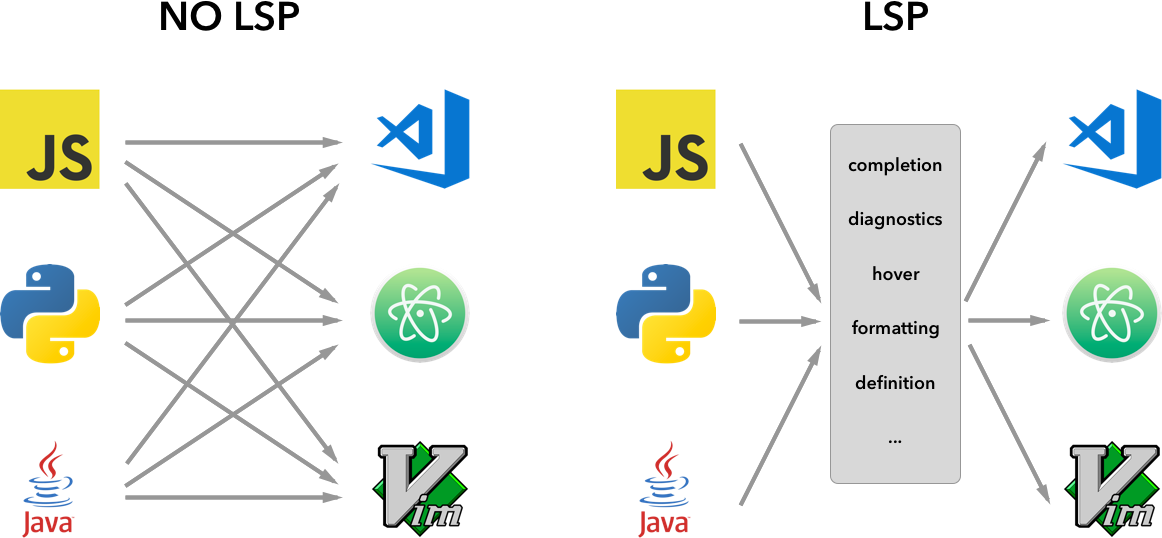
\includegraphics[width=0.7\textwidth]{figs/LSP-MxN.png}
  \label{figure:lsp}
  \caption{
    The motivation behind LSP, from Microsoft's website.
    \protect\footnotemark
  }
\end{figure}
\footnotetext{\raggedright\url{https://code.visualstudio.com/api/language-extensions/language-server-extension-guide}}

This protocol is particularly useful for interactive theorem provers since
they rely on the editing experience much more than a command line interface.
This is due to the fact that theorem provers generally do not need to compile
to any kind of executable file and only need the type-checking stage of compilers,
which can be easily performed by a language server. However, this also adds extra work
on the language server since it needs to support more features than a regular compiler would,
including listing variables in context along with their types, supporting Unicode symbols,
and most importantly allowing for an interactive step-by-step proof walkthrough.

\section{Related Work}

% \subsection{Language Server Protocol}
% The Language Server protocol was developed by Microsoft in an effort to decouple a language's implementation from its editor interface \cite{Buender2019}. It has contributed significantly to decreasing the effort required to add support for a given programming language in a given text editor (that supports LSP).

\subsubsection{Specification Language Server Protocol.}

While LSP has greatly improved the experience of developing language servers,
it still leaves a bit to be desired.
LSP was mainly designed with general purpose programming languages in mind,
but theorem provers (or more generally, specification language) have slightly
different requirements that are unmet by LSP.
This is why \cite{JonasKjaerRask2021} attempts to extend the original LSP
specification with features that are especially useful for specification languages.
The authors call the protocol extension \textit{Specification Language Server Protocol} (SLSP).
Simply speaking, it defines a set of new LSP requests/notification along with
their payloads, and extends VS Code's interface with a view that displays proof
information in a way similar to Proof General \cite{Aspinall2000}.

\subsubsection{VS Code extension for Lean 4.}

Lean 4 \cite{deMouraUllrich2021} is a programming language and proof assistant
by Microsoft Research\footnote{\url{https://www.microsoft.com/en-us/research/project/lean/}}
from which we draw much inspiration.
In particular, the primary way to develop Lean programs is using its VS Code
extension that provides a user interface for working with Lean interactively.
This extension uses LSP to communicate with the Lean server and provides a lot
of useful features, the most notable of which is the Info View panel that
displays information about current proof state and allows interacting with it \cite{Nawrocki2023}.

\subsubsection{Proof General.}

Proof General \cite{Aspinall2000} is a tool for developing interactive theorem
provers that has been used for many widely-known proof assistants such as Coq
and Isabelle.
It is based on the Emacs editor and provides an interactive GUI with relative
ease for theorem provers developed with its help.
% The interface produced by Proof General is familiar to many users of theorem
% provers, and so it makes sense to use it as a reference when developing the
% interface of a new proof assistant.

% \subsection{Libraries for proof assistant development}

% \nikolai{We should mention the A.L.G.A.E. project: \url{https://redprl.org/#algae}}
% \abdelrahman{Seems like largely a work in progress. I don't see how we can use any of the libraries mentioned there.}

\section{Contribution}

In this paper, we report on the work-in-progress on the implementation of
utility and interactive tools around \Rzk{} proof assistant, focusing on
the language server and VS Code extension support.
